\documentclass[notes,10pt, aspectratio=169]{beamer}

\usepackage{pgfpages}
% These slides also contain speaker notes. You can print just the slides,
% just the notes, or both, depending on the setting below. Comment out the want
% you want.
\setbeameroption{hide notes} % Only slide
%\setbeameroption{show only notes} % Only notes
%\setbeameroption{show notes on second screen=right} % Both
\usepackage{wrapfig}

\usepackage{helvet}
\usepackage[default]{lato}
\usepackage{array}
\usepackage{eurosym}
\usepackage{setspace}
\usepackage{animate}
\usepackage{multicol}
\usepackage{breqn}
\usepackage{subcaption}
\usepackage{caption}
\captionsetup{font=scriptsize, justification=raggedright,singlelinecheck=false}
\usepackage[export]{adjustbox}
\usepackage[scale=2]{ccicons}
\usepackage{tikz}
\newenvironment{wideitemize}{\itemize\addtolength{\itemsep}{10pt}}{\enditemize}
\usepackage{natbib}

\usepackage{tikz}
\usepackage{verbatim}
\setbeamertemplate{note page}{\pagecolor{yellow!5}\insertnote}
\usepackage{amsmath}
%\usepackage{mathpazo}
\usepackage{hyperref}
\usepackage{lipsum}
\usepackage{multimedia}
\usepackage{multirow}
\usepackage{graphicx}
\usepackage{dcolumn}
\usepackage{bbm}
\newcolumntype{d}[0]{D{.}{.}{5}}

\usepackage{changepage}
\usepackage{appendixnumberbeamer}
% \newcommand{\beginbackup}{
%   \newcounter{framenumbervorappendix}
%   \setcounter{framenumbervorappendix}{\value{framenumber}}
%   \setbeamertemplate{footline}
%   {
%      \leavevmode%
%      \hline
%      box{%
%       \begin{beamercolorbox}[wd=\paperwidth,ht=2.25ex,dp=1ex,right]{footlinecolor}%
% %         \insertframenumber  \hspace*{2ex} 
%       \end{beamercolorbox}}%
%      \vskip0pt%
%   }
%  }
\useinnertheme[shadow]{rounded}
\setbeamercolor{block title example}{fg=black,bg=orange!50!white}
\setbeamercolor{block body example}{fg=black, bg=orange!30!white}
\setbeamercolor{block title}{use=structure,fg=structure.fg,bg=structure.fg!20!bg}
\setbeamercolor{block body}{parent=normal text,use=block title,bg=block title.bg!50!bg}

 \setbeamertemplate{footline}{
    \hbox{%
    \begin{beamercolorbox}[wd=\paperwidth,ht=3ex,dp=1.5ex,leftskip=2ex,rightskip=2ex]{page footer}%
        %\usebeamerfont{title in head/foot}%
        %\insertshorttitle \hfill
        %\insertsection \hfill
        %\tableofcontents[currentsection] \hfill
        \insertsectionnavigationhorizontal{0.7\paperwidth}{}{} \hfill 
        \insertframenumber{} / \inserttotalframenumber
    \end{beamercolorbox}}%
}
\newcommand{\backupend}{
   \addtocounter{framenumbervorappendix}{-\value{framenumber}}
   \addtocounter{framenumber}{\value{framenumbervorappendix}} 
}


\usepackage{graphicx}
\usepackage[space]{grffile}
\usepackage{booktabs}

% These are my colors -- there are many like them, but these ones are mine.
\definecolor{blue}{RGB}{0,114,178}
\definecolor{red}{RGB}{213,94,0}
\definecolor{yellow}{RGB}{240,228,66}
\definecolor{green}{RGB}{0,158,115}

\setbeamercolor{section in head/foot}{fg=blue}


\hypersetup{
  colorlinks=false,
  linkbordercolor = {white},
  linkcolor = {blue}
}


%% I use a beige off white for my background
\definecolor{MyBackground}{RGB}{255,253,218}

%% Uncomment this if you want to change the background color to something else
%\setbeamercolor{background canvas}{bg=MyBackground}

%% Change the bg color to adjust your transition slide background color!
\newenvironment{transitionframe}{
  \setbeamercolor{background canvas}{bg=yellow}
  \begin{frame}}{
    \end{frame}
}

\setbeamercolor{frametitle}{fg=blue}
\setbeamercolor{title}{fg=black}
%\setbeamertemplate{footline}[frame number]
\setbeamertemplate{navigation symbols}{} 
\setbeamertemplate{itemize items}{-}
\setbeamercolor{itemize item}{fg=blue}
\setbeamercolor{itemize subitem}{fg=blue}
\setbeamercolor{enumerate item}{fg=blue}
\setbeamercolor{enumerate subitem}{fg=blue}
\setbeamercolor{button}{bg=white,fg=blue,}



% If you like road maps, rather than having clutter at the top, have a roadmap show up at the end of each section 
% (and after your introduction)
% Uncomment this is if you want the roadmap!
% \AtBeginSection[]
% {
%    \begin{frame}
%        \frametitle{Roadmap of Talk}
%        \tableofcontents[currentsection]
%    \end{frame}
% }
\setbeamercolor{section in toc}{fg=blue}
\setbeamercolor{subsection in toc}{fg=red}
%\setbeamersize{text margin left=1em,text margin right=1em} 
\setbeamersize{text margin left=0.7cm,text margin right=0.7cm} 


\title[]{\textcolor{blue}{Lecture 3:\\Simple Linear Regression}}
\author{25117 - Econometrics}
\institute[shortinst]{Universitat Pompeu Fabra}

\date{October 7th, 2024}

\begin{document}



% Title Slide

\begin{frame}[plain]
\maketitle
\end{frame}

\section{Introduction}

\begin{frame}{What we learned in the last lesson}
\begin{itemize}
    \item The sample average, $\overline{Y}$, is an estimator of the population mean, $\mu_Y$. When $Y_1, \dots ,Y_n$ are i.i.d.,
    \begin{enumerate}
        \item  The sampling distribution of $\overline{Y}$ has mean $\mu_Y$ and variance $\sigma_{\overline{Y}}^2=\sigma_Y^2/n$
        \item $\overline{Y}$ is unbiased
        \item by the LLN, $\overline{Y}$ is consistent; and
        \item by the CLT, $\overline{Y}$ has an approximately normal sampling distribution when the $n$ is large.
    \end{enumerate}
    \item The t-statistic is used to test the null hypothesis that the population mean takes on a particular value. If $n$ is large, the t-stat $\sim \mathcal{N}(0,1)$ under $H_0$.
    \item The t-statistic can be used to calculate the p-value associated with the null hypothesis. The p-value is the probability of drawing a statistic at least as adverse to the null hypothesis as the one you actually computed in your sample, assuming the null hypothesis is correct. A small p-value is evidence that the null hypothesis is false.
    \item A 95\% confidence interval for $\mu_Y$ contains the true value of $\mu_Y$ in 95\% of all possible samples.
    \item The sample correlation coefficient is an estimator of the population correlation coefficient and measures the linear relationship between two variables -- that is, how well their scatterplot is approximated by a straight line.
\end{itemize}
\end{frame}


\begin{frame}{The regression line}
 \begin{columns}
\begin{column}{0.35\textwidth}
    \begin{itemize}
        \item The population regression line is the expected value of Y given X.
        \item The slope is the difference in the expected values of Y, for two values of X that differ by one unit
    \end{itemize}
\end{column}
\begin{column}{0.7\textwidth}
\begin{figure}
  \centering
         \vspace{-1mm}
        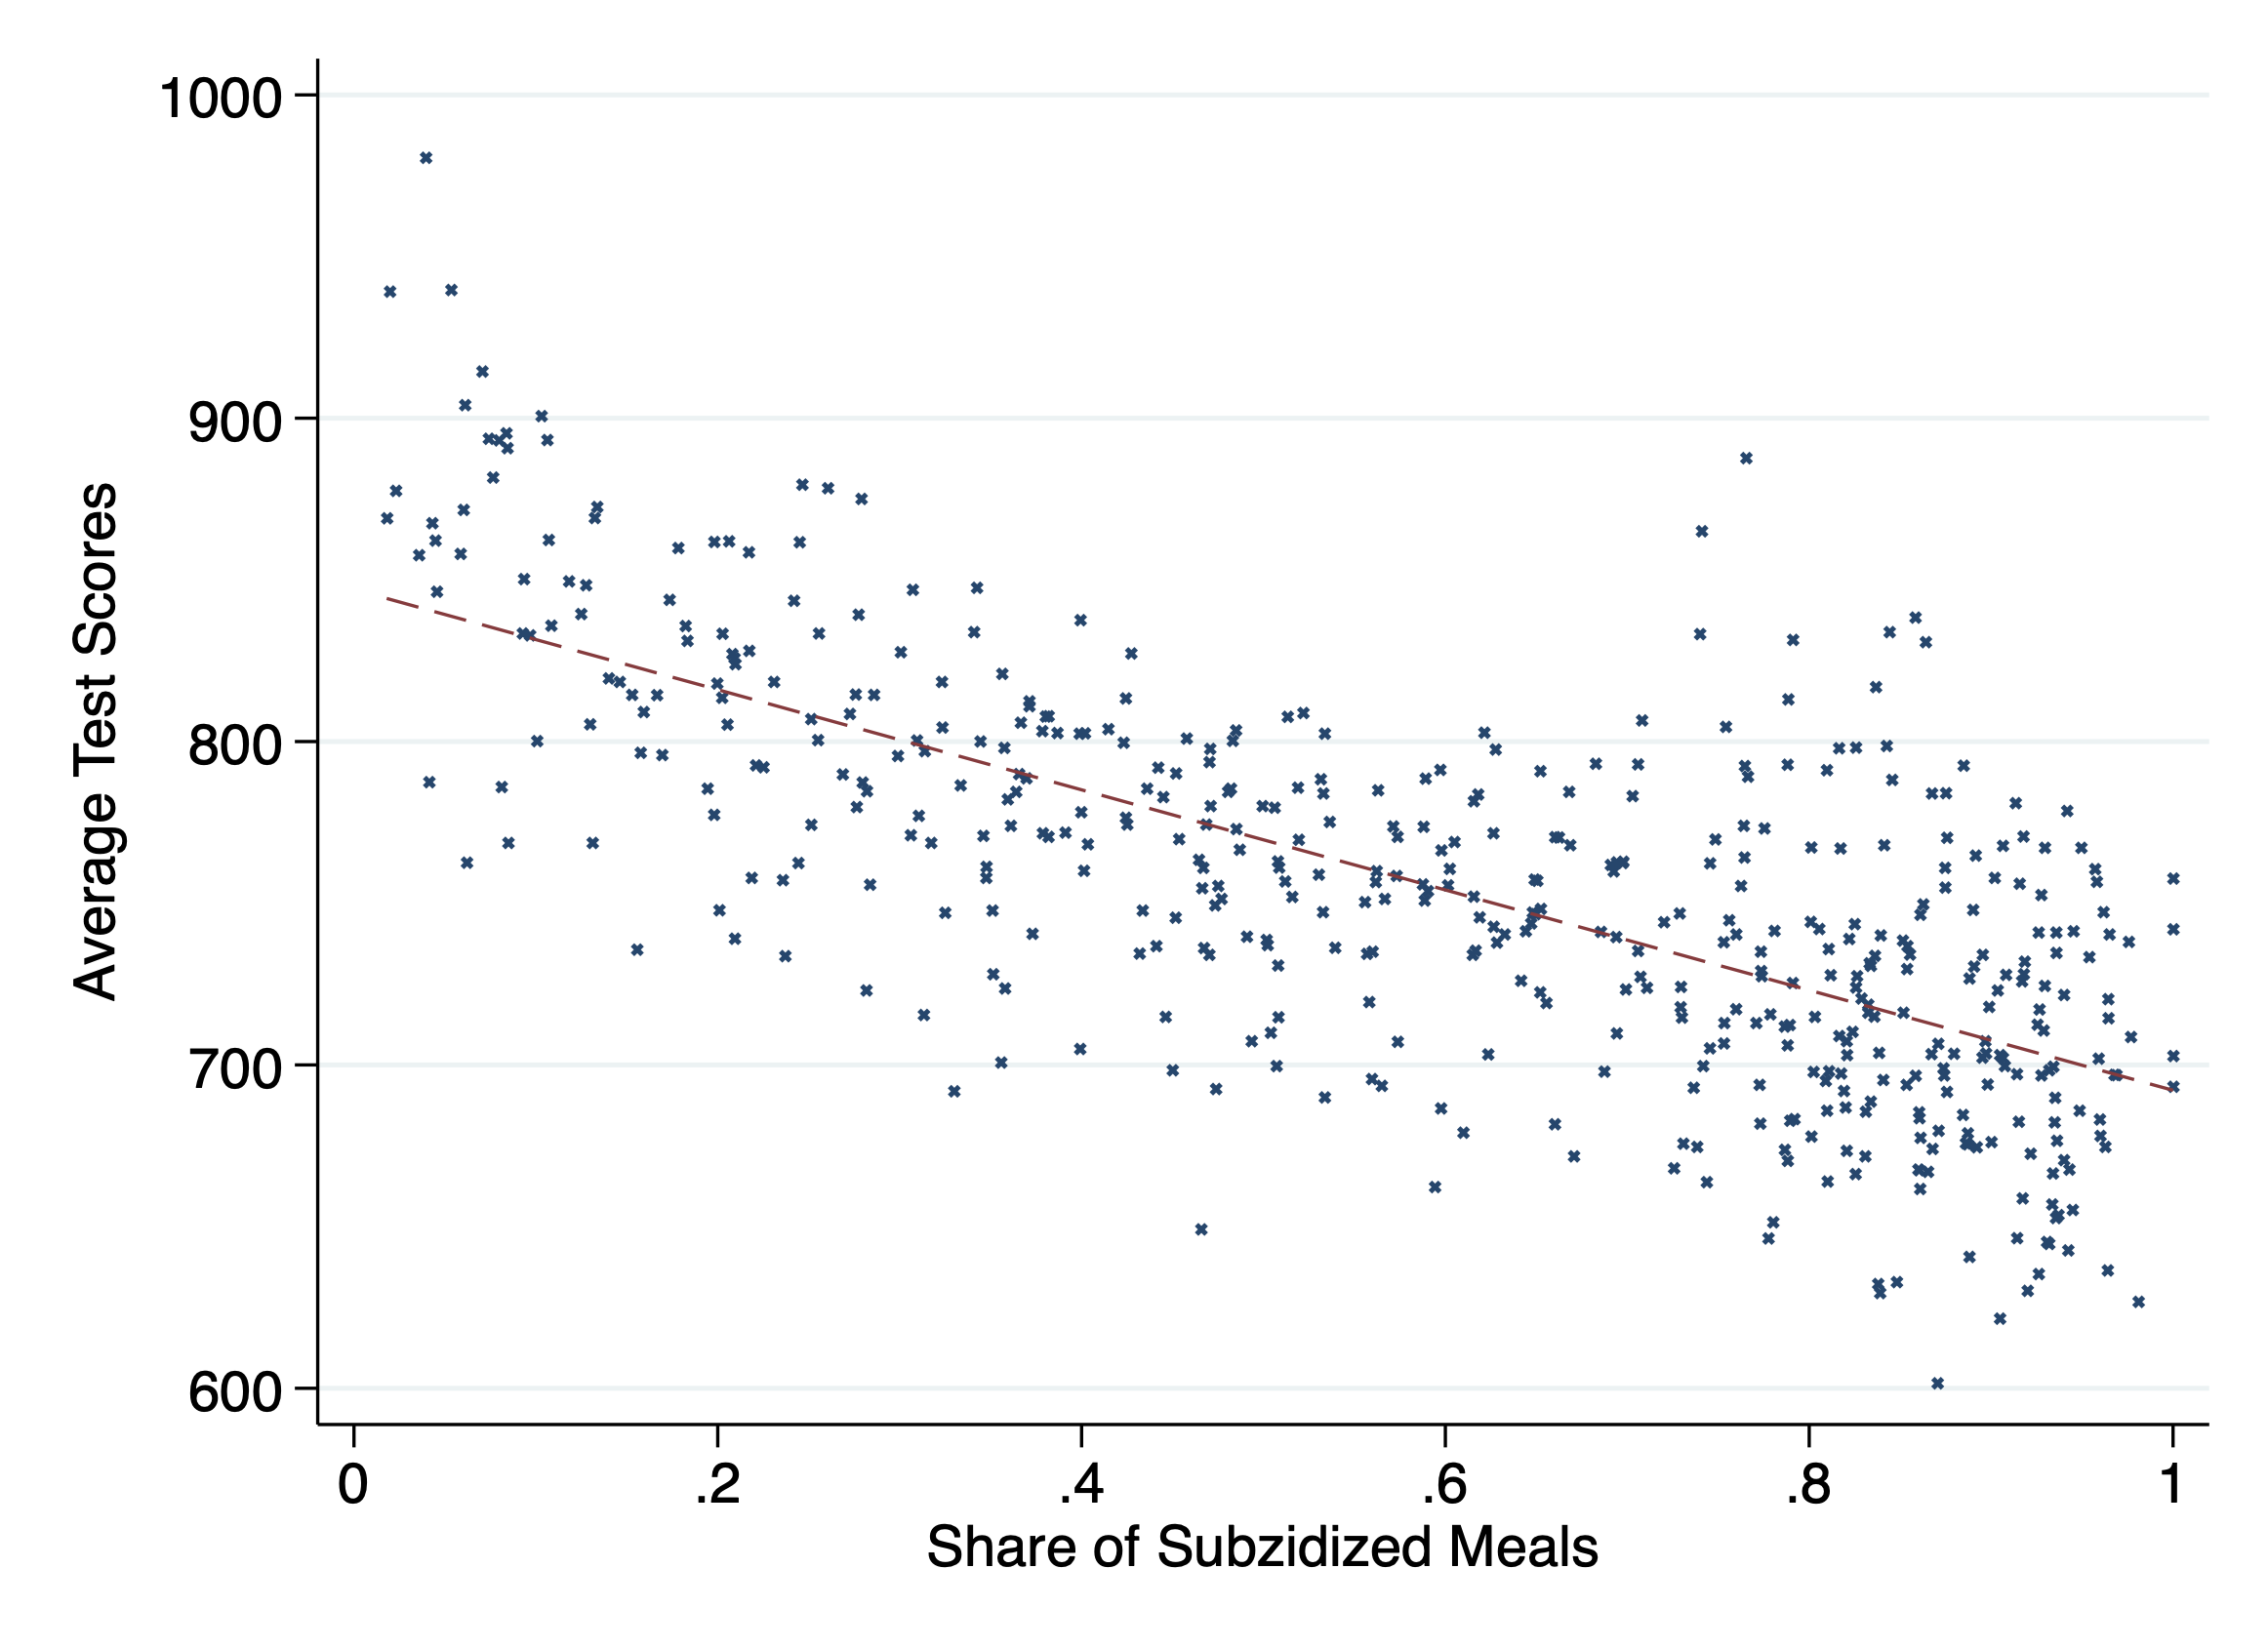
\includegraphics[scale=.25]{images/testscores_corr.png}
\end{figure}
\end{column}
\end{columns}
\end{frame}



\begin{frame}{The regression line}
 \begin{columns}
\begin{column}{0.35\textwidth}
 The estimated regression can be used either for
        \begin{enumerate}
            \item \textbf{causal inference} (learning about the causal effect on Y of a change in X)
            \begin{itemize}
                \item[$\rightarrow$] What is the causal impact of subsidizing meals on students' performances?
            \end{itemize}
            \item \textbf{prediction} (predicting the value of Y given X, for an observation not in the data set)
            \begin{itemize}
                \item[$\rightarrow$] What are the students' expected test scores given the share of subsidized meals?
            \end{itemize}
        \end{enumerate}
\end{column}
\begin{column}{0.7\textwidth}
\begin{figure}
  \centering
         \vspace{-1mm}
        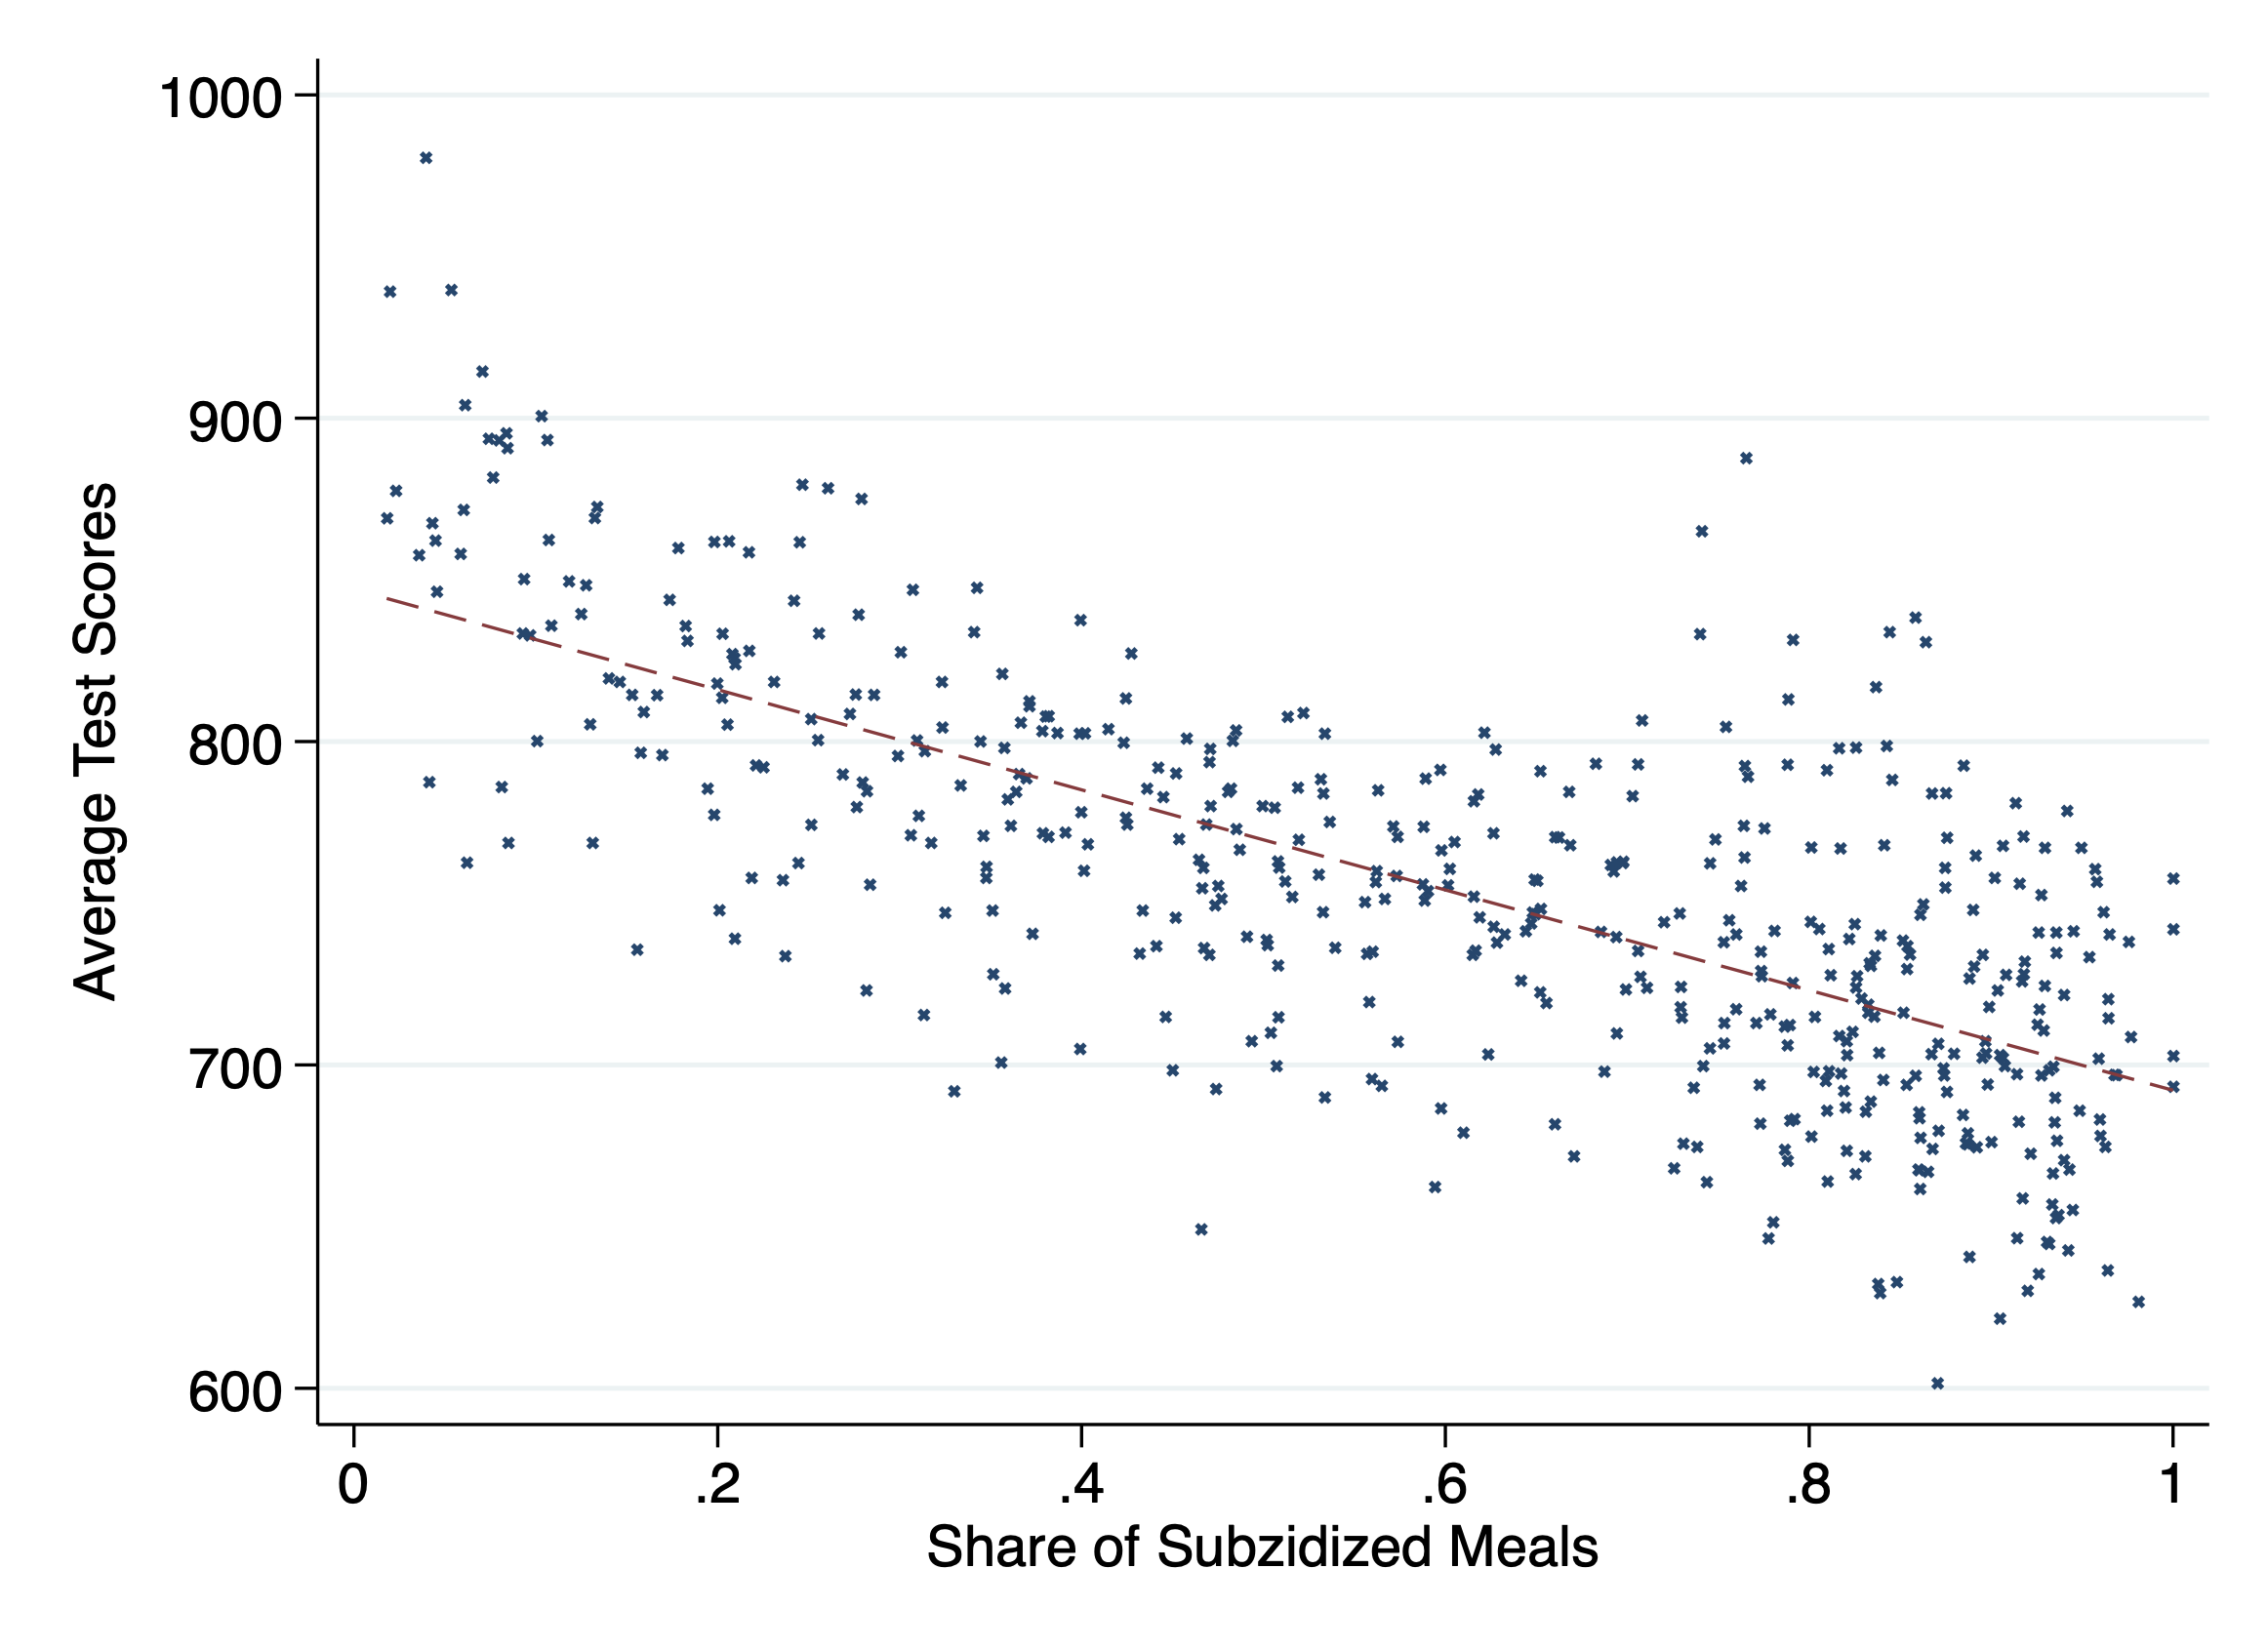
\includegraphics[scale=.25]{images/testscores_corr.png}
\end{figure}
\end{column}
\end{columns}
\end{frame}


\begin{frame}{The Population Linear Regression Model}
 \begin{columns}
\begin{column}{0.35\textwidth}
\begin{equation*}
    Y_i¨ = \beta_0 + \beta_1 X_i + u_i
\end{equation*}
\begin{itemize}
    \item There are $n$ observations, $(X_i,Y_i)$, $i=\{1,\dots, n\}$
    \item $Y$ is the dependent variable
    \item $X$ is the independent variable or regressor
    \item $\mathbb{E}(Y\mid X) = \beta_0 + \beta_1 X$ is the population regression line
    \item $\beta_0$ is called the intercept
    \item $\beta_1$ is the slope
    \item $u_i$ is the error term
\end{itemize}
\end{column}
\begin{column}{0.7\textwidth}
\begin{figure}
  \centering
         \vspace{-1mm}
        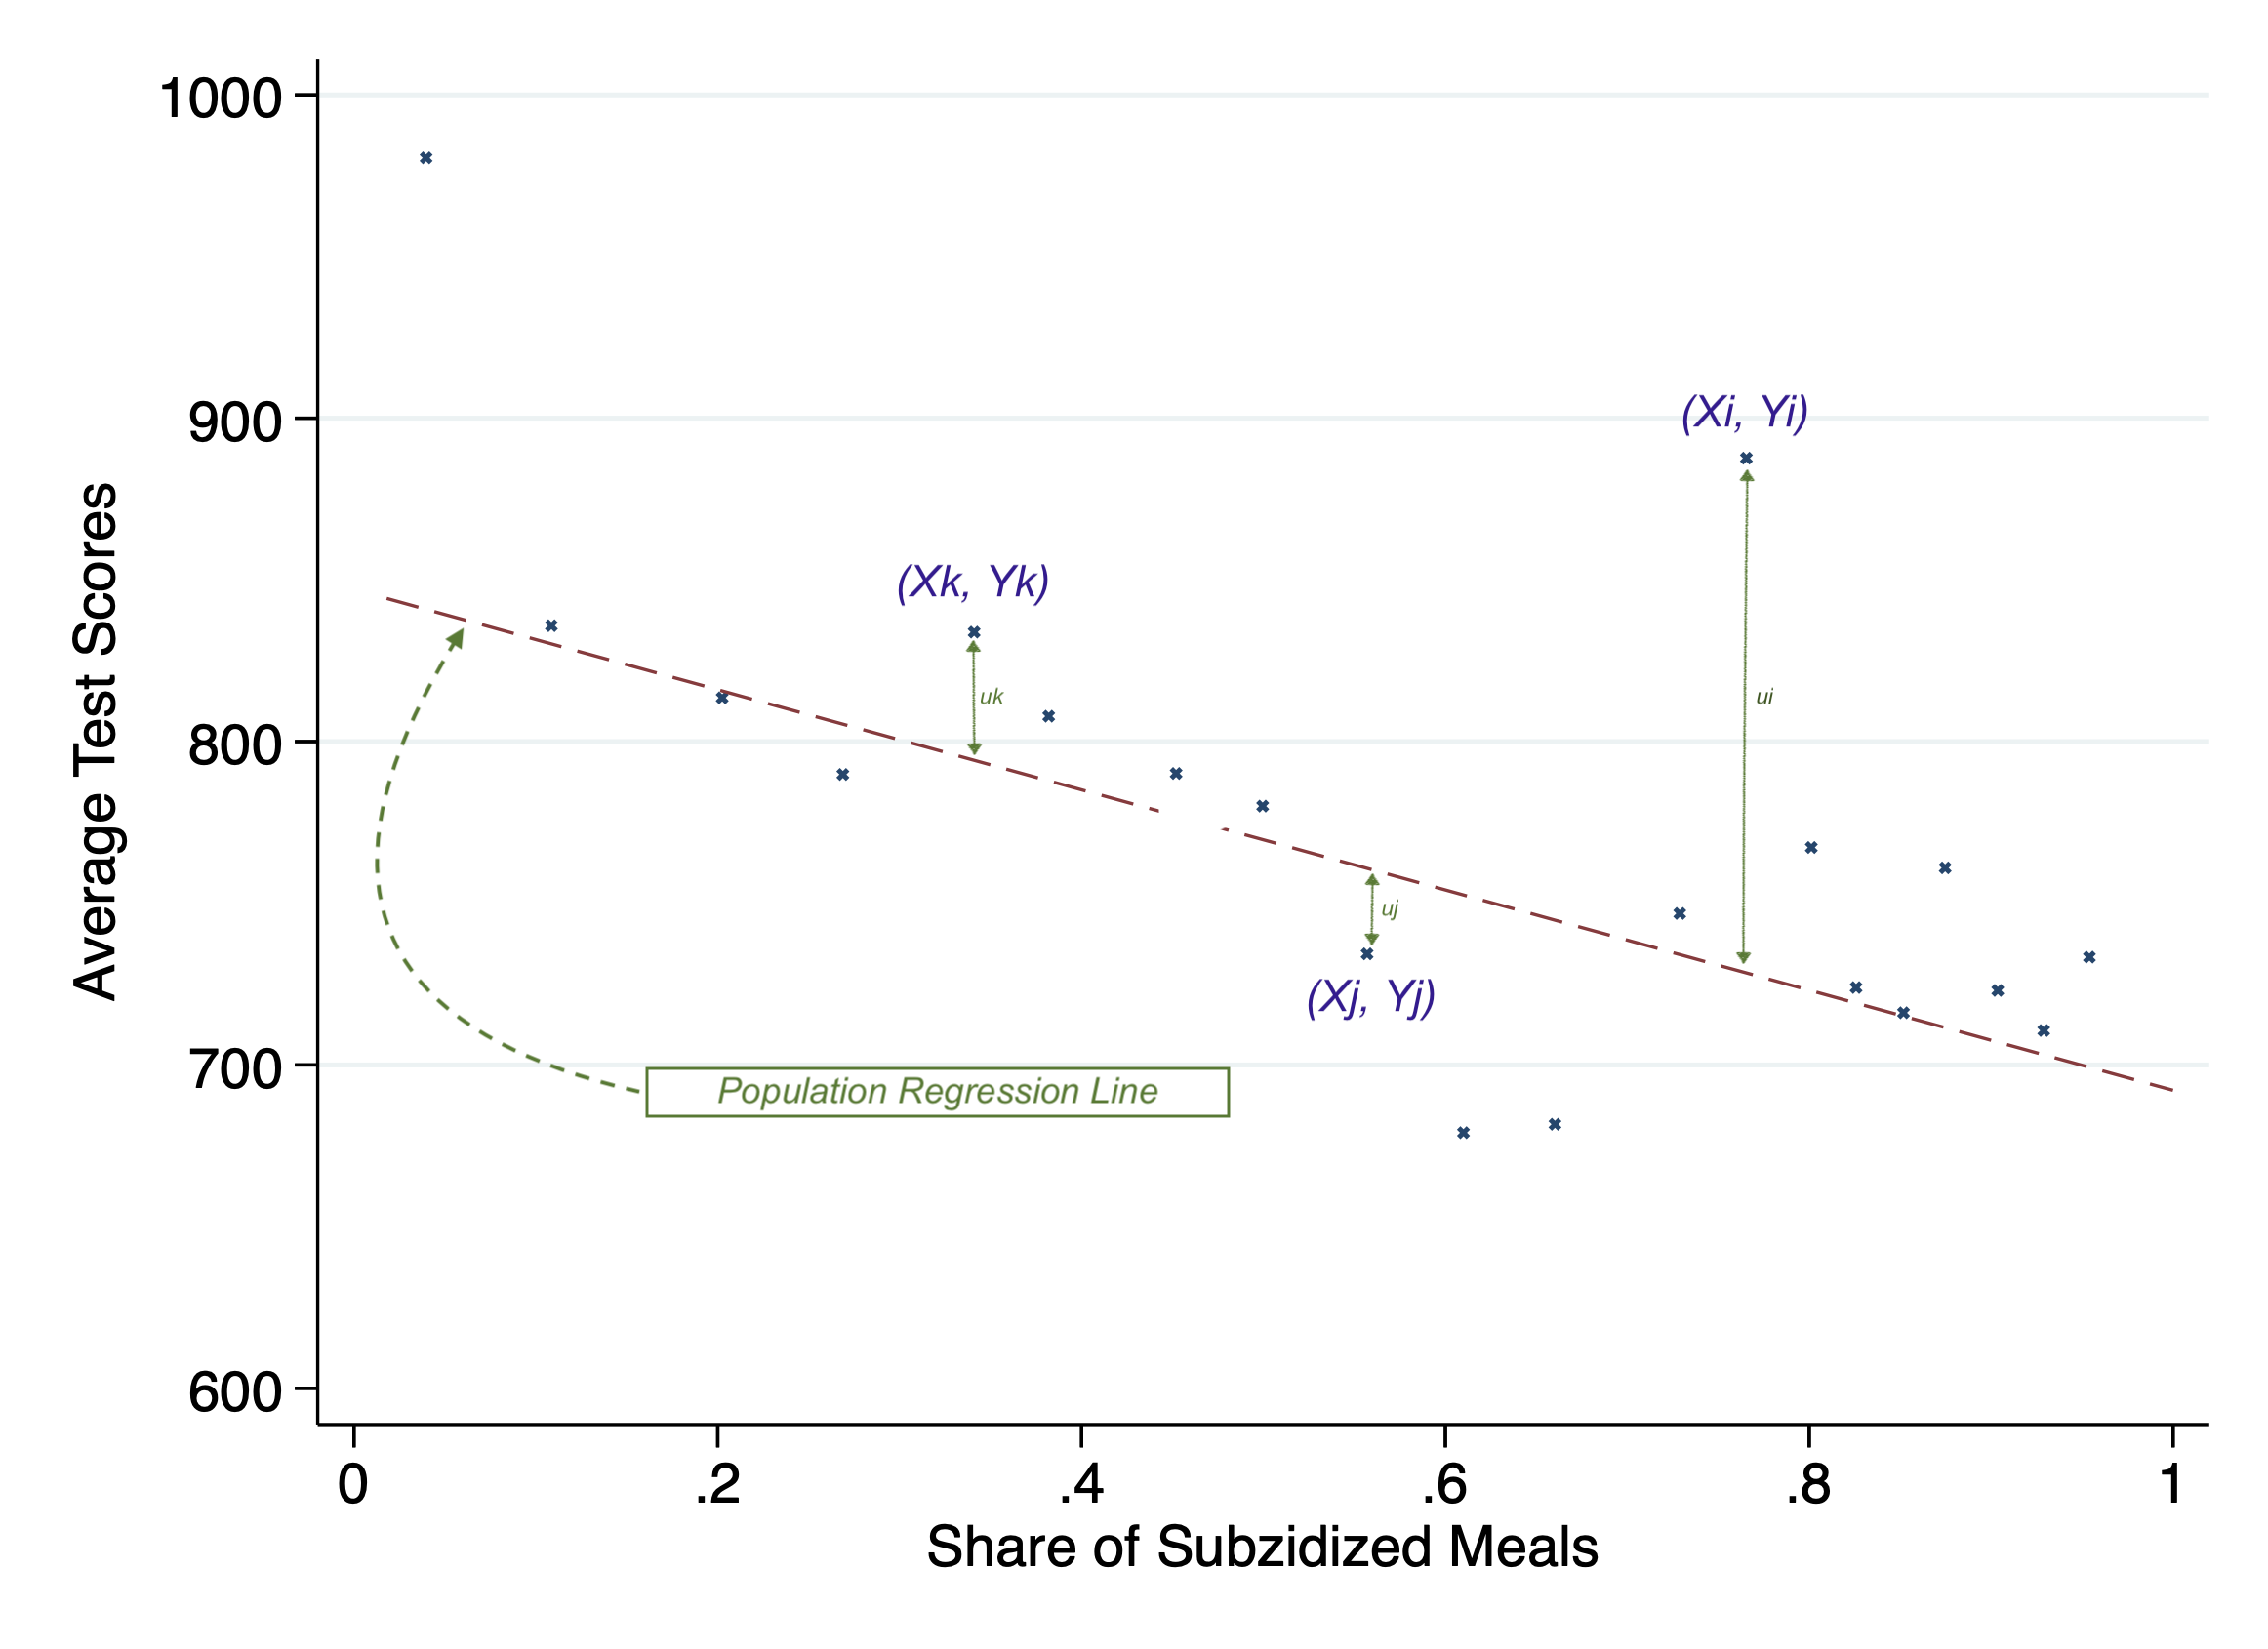
\includegraphics[scale=.25]{images/regression0.png}
\end{figure}
\end{column}
\end{columns}
\end{frame}



\begin{frame}{The Ordinary Least Squares (OLS) Estimator}
How can we estimate $\beta_0$ and $\beta_1$ from the data? Recall from Lecture 1 that the Least Square estimator of $\mu_Y$, $\overline{Y}$, solves
\begin{equation*}
    \min_m \sum_{i=1}^n (Y_i - m)^2
\end{equation*}
\\
By analogy, the OLS estimators of the unknown parameters $\beta_0$ and $\beta_1$,  $\hat{\beta}_0$ and $\hat{\beta}_1$ solves,
\begin{eqnarray*}
    &  &\min_{\beta_0, \beta_1} \sum_{i=1}^n u_i^2\\
    & \Leftrightarrow &\min_{\beta_0, \beta_1} \sum_{i=1}^n (Y_i - \mathbb{E}(Y\mid X))^2\\
   & \Leftrightarrow &\min_{\beta_0, \beta_1} \sum_{i=1}^n (Y_i - (\hat{\beta}_0 + \hat{\beta}_1 X_i))^2
\end{eqnarray*}
\end{frame}


\begin{frame}{The Ordinary Least Squares (OLS) Estimator}
\begin{eqnarray*}
    &\begin{cases}
    \frac{\partial}{\partial \beta_0} \sum_{i=1}^n (Y_i - (\hat{\beta}_0 + \hat{\beta}_1 X_i))^2 = 0\\
    \frac{\partial}{\partial \beta_1} \sum_{i=1}^n (Y_i - (\hat{\beta}_0 + \hat{\beta}_1 X_i))^2 = 0
    \end{cases}\\ 
    \Rightarrow
    &\begin{cases}
    -2 \sum_{i=1}^n (Y_i - (\hat{\beta}_0 + \hat{\beta}_1 X_i)) = 0\\
    -2 \sum_{i=1}^n (Y_i - (\hat{\beta}_0 + \hat{\beta}_1 X_i))X_i = 0
    \end{cases}\\ 
    \Rightarrow
    &\begin{cases}
    \frac{1}{n}\sum_{i=1}^n Y_i - \frac{1}{n}\sum_{i=1}^n\hat{\beta}_0 -\frac{1}{n}\sum_{i=1}^n \hat{\beta}_1 X_i = 0\\
    \frac{1}{n}\sum_{i=1}^n Y_iX_i - \frac{1}{n}\sum_{i=1}^n\hat{\beta}_0X_i -\frac{1}{n}\sum_{i=1}^n \hat{\beta}_1 X_i^2 = 0
    \end{cases}\\ 
    \Rightarrow
    &\begin{cases}
    \overline{Y} - \hat{\beta}_0 -\hat{\beta}_1 \overline{X} = 0\\
    \frac{1}{n}\sum_{i=1}^n Y_iX_i - \hat{\beta}_0 \overline{X} - \hat{\beta}_1  \frac{1}{n}\sum_{i=1}^n X_i^2 = 0
    \end{cases}\\ 
\end{eqnarray*}
\end{frame}

\begin{frame}{The Ordinary Least Squares (OLS) Estimator}
\begin{eqnarray*}
        \Rightarrow
    &\begin{cases}
    \hat{\beta}_0 = \overline{Y}  -\hat{\beta}_1 \overline{X}\\
    \frac{1}{n}\sum_{i=1}^n Y_iX_i - \overline{Y}\overline{X} - \hat{\beta}_1( \frac{1}{n}\sum_{i=1}^n X_i^2 - \overline{X}\overline{X}) = 0
    \end{cases}\\ 
    \Rightarrow
    &\begin{cases}
    \hat{\beta}_0 = \overline{Y}  -\hat{\beta}_1 \overline{X}\\
    \hat{\beta}_1= \frac{\frac{1}{n}\sum_{i=1}^n Y_iX_i - \overline{Y}\overline{X}}{\frac{1}{n}\sum_{i=1}^n X_i^2 - \overline{X}\overline{X}}
    \end{cases}\\ 
        \Rightarrow
    &\begin{cases}
    \hat{\beta}_0 = \overline{Y}  -\hat{\beta}_1 \overline{X}\\
    \hat{\beta}_1= \frac{\frac{1}{n}\sum_{i=1}^n (Y_i-\overline{Y})(X_i - \overline{X})}{\frac{1}{n}\sum_{i=1}^n (X_i - \overline{X})^2}
    \end{cases}\\ 
     \Rightarrow
    &\begin{cases}
    \hat{\beta}_0 = \overline{Y}  -\hat{\beta}_1 \overline{X}\\
    \hat{\beta}_1= \frac{s_{XY}}{s^2_{X}}
    \end{cases}\\
\end{eqnarray*}

\end{frame}



\begin{frame}{Back to the Linear Regression Model}
 \begin{columns}
\begin{column}{0.35\textwidth}
The OLS estimator minimizes the average squared difference between the actual values of i Y and the prediction (“predicted value”) based on the estimated line.
\begin{itemize}
    \item $\hat{\beta}_0 = \overline{Y}  -\hat{\beta}_1 \overline{X}$
    \item $\hat{\beta}_1= \frac{s_{XY}}{s^2_{X}}$
    \item $\hat{Y}_i = \hat{\beta}_0 + \hat{\beta}_1X_i$
    \item $\hat{u_i} = Y_i - \hat{Y}_i$
\end{itemize}
This means that
\begin{itemize}
    \item $\Delta\mathbb{E}(Y_i\mid X_i) = \hat{\beta}_1\Delta X_i$
\end{itemize}s
\end{column}
\begin{column}{0.7\textwidth}
\begin{figure}
  \centering
         \vspace{-1mm}
        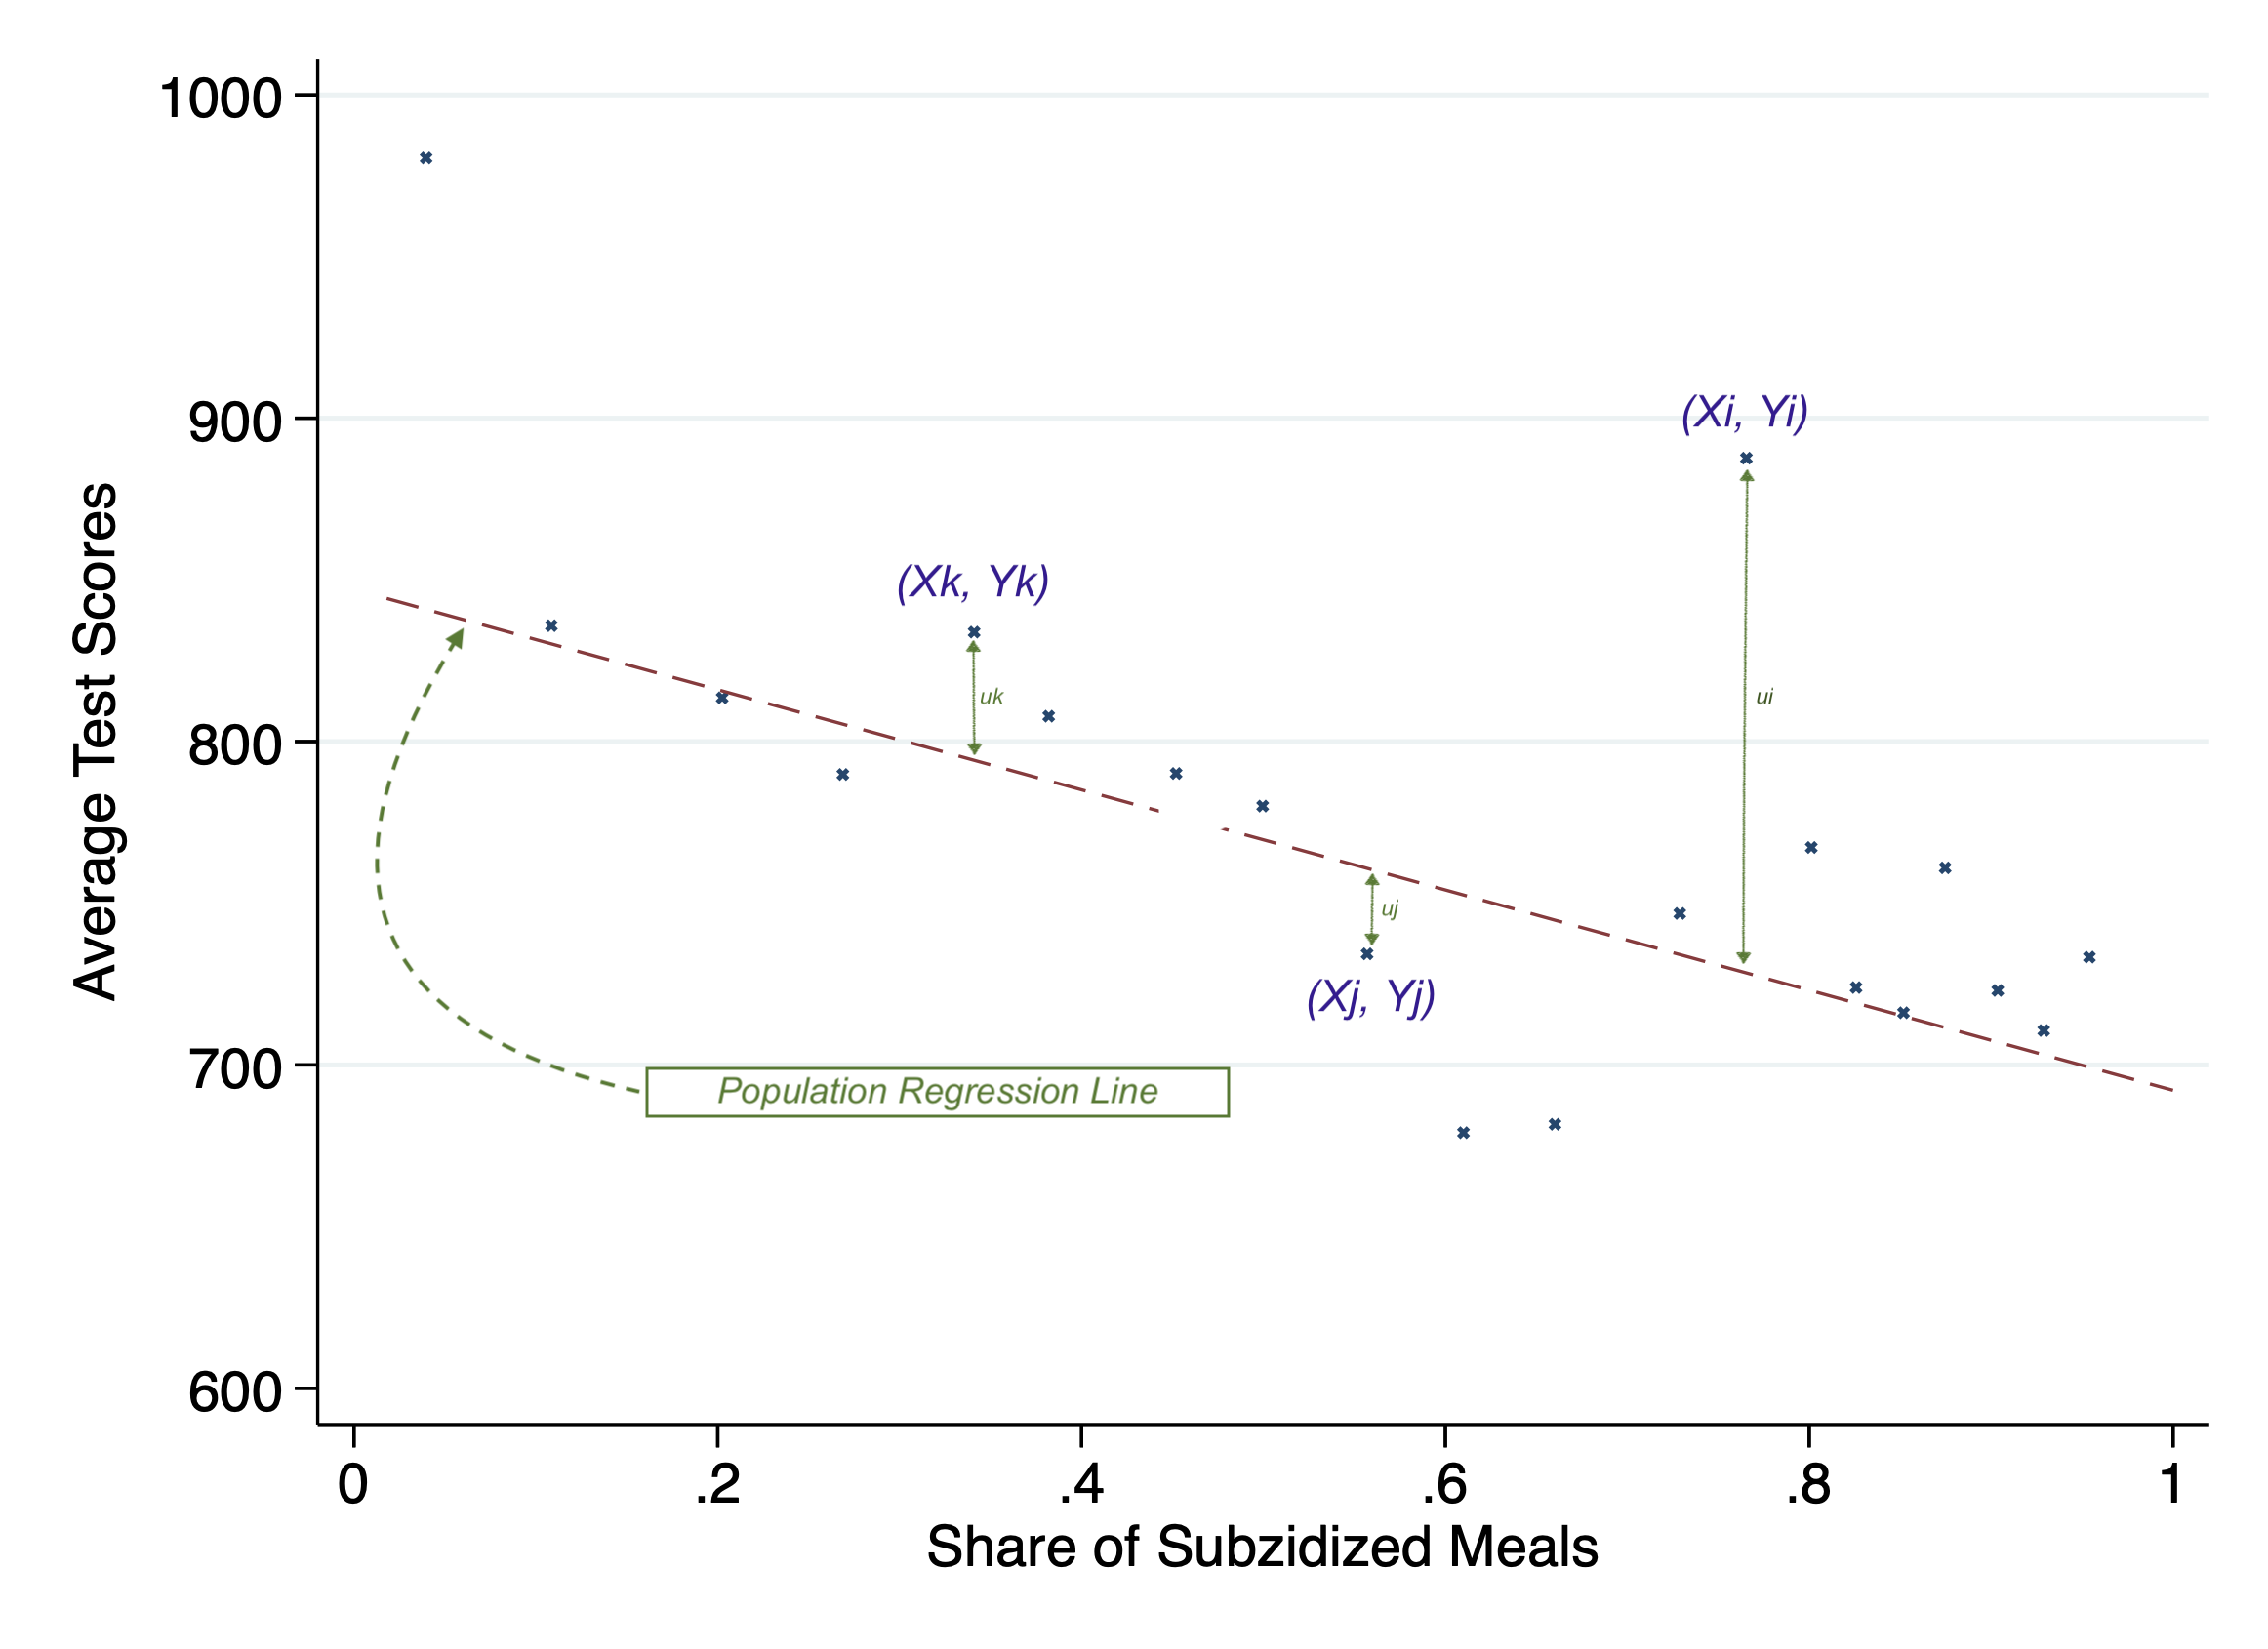
\includegraphics[scale=.25]{images/regression0.png}
\end{figure}
\end{column}
\end{columns}
\end{frame}


\begin{frame}{Interpretation}
Here, the population regression line is given by
\begin{eqnarray*}
     \hat{\beta}_0 \approx 754+155\times.6 \approx 847\\
     \hat{\beta}_1 \approx \frac{ -11.78}{.28^2} \approx -155\\
    \hat{Y}_i \approx 847 -155\times X_i
\end{eqnarray*}
\begin{itemize}
    \item This means that a 10ppt increase in the share of subsidized meals is associated with ($\neq$ cause!) a 15.5 decrease in the average test scores. 
    \item To give a standard of comparison, this is about 26\% of the Test scores' standard deviation!
    \item The intercept (taken literally) means that, according to this estimated line, districts with zero meals would have a (predicted) test score of approximately 847...
    \item But this interpretation of the intercept makes no sense -- it extrapolates the line outside the range of the data (see Lect2 for descriptive stats) -- here, the intercept is not economically meaningful.
\end{itemize}
\end{frame}


\begin{frame}{Goodness of Fit}
\begin{itemize}
\item How well does our regression model fit the data? This is a crucial question.
\item Goodness of fit measures help us assess the quality of our model.
\item Two regression statistics provide complementary measures of how well the regression line “fits” or explains the data:
\begin{enumerate}
    \item The regression $R^2$ measures the fraction of the variance of Y that is explained by X; it is unitless and ranges between zero (no fit) and one (perfect fit)
    \item The standard error of the regression ($SER$) measures the magnitude of a typical regression residual in the units of Y.
\end{enumerate}
\item These measures are very useful to predict $Y$ when $X$ is known but $Y$ is not (out-of-sample prediction). A common prediction measure is $\hat{Y}\pm SER$.
\end{itemize}
\end{frame}


\begin{frame}{$R^2$}
From the previous slides, we note that
\begin{equation*}
    Y_i = \hat{Y}_i + \hat{u}_i
\end{equation*}
The $R^2$ is the ratio of the sample variance of $\hat{Y}$ to the sample variance of $Y$
\begin{eqnarray*}
    &R^2 &= \frac{\text{explained sum of squares ($ESS$)}}{\text{total sum of squares ($TSS$)}} = \frac{\sum_{i=1}^n (\hat{Y}_i - \overline{Y})^2}{\sum_{i=1}^n (Y_i - \overline{Y})^2}\\
    & &= 1-\frac{\text{sum of squared residuals ($SSR$)}}{\text{total sum of squares ($TSS$)}} = 1-\frac{\sum_{i=1}^n \hat{u}_i^2}{\sum_{i=1}^n (Y_i - \overline{Y})^2}
\end{eqnarray*}
$R^2$ ranges from 0 to 1, where higher values indicate a better fit (i.e., the regressor is good at predicting the outcome)
\end{frame}



\begin{frame}{The Standard Error of the Regression ($SER$)}
The SER measures the spread of the distribution of $u$ around the regression line in the units of the dependent variable.
It is an estimator of the standard deviation of the regression error $u_i$.
\begin{equation*}
    SER = \sqrt{\frac{1}{n-2}\sum_{i=1}^n (\hat{u}_i-\overline{\hat{u}}_i)^2}= \sqrt{\frac{1}{n-2}\sum_{i=1}^n \hat{u}_i^2}=\sqrt{\frac{SSR}{n-2}}
\end{equation*}
Here, division by $n-2$ is a dof correction (two parameters, $\beta_0$ and $\beta_1$ have been estimated, whereas in $s_Y^2$ only one has been estimated: $\mu_Y$, with $\overline{Y}$)\\\vspace{.5cm}
The root mean squared error ($RMSE$) is closely related to the $SER$:
\begin{equation*}
    RMSE = \sqrt{\frac{SSR}{n}}
\end{equation*}
In practice, that does not change anything for large samples. Both are interesting as they provide a consistent estimate of the standard deviation in the unobservables affecting $Y$. 
\end{frame}


\begin{frame}{Goodness of Fit}
 \begin{columns}
\begin{column}{0.35\textwidth}
\begin{itemize}
    \item Here the $R^2=.509$ and $RMSE=42.601$
    \item About half of the variation in actual test scores is explained by the variation in the predicted test scores (which, in our regression specification, comes from the variation in subsidized meals).
    \item Does this make sense? Does this mean that subsidizing school meals matters for education in a policy sense?
\end{itemize}
\end{column}
\begin{column}{0.7\textwidth}
\begin{figure}
  \centering
         \vspace{-1mm}
        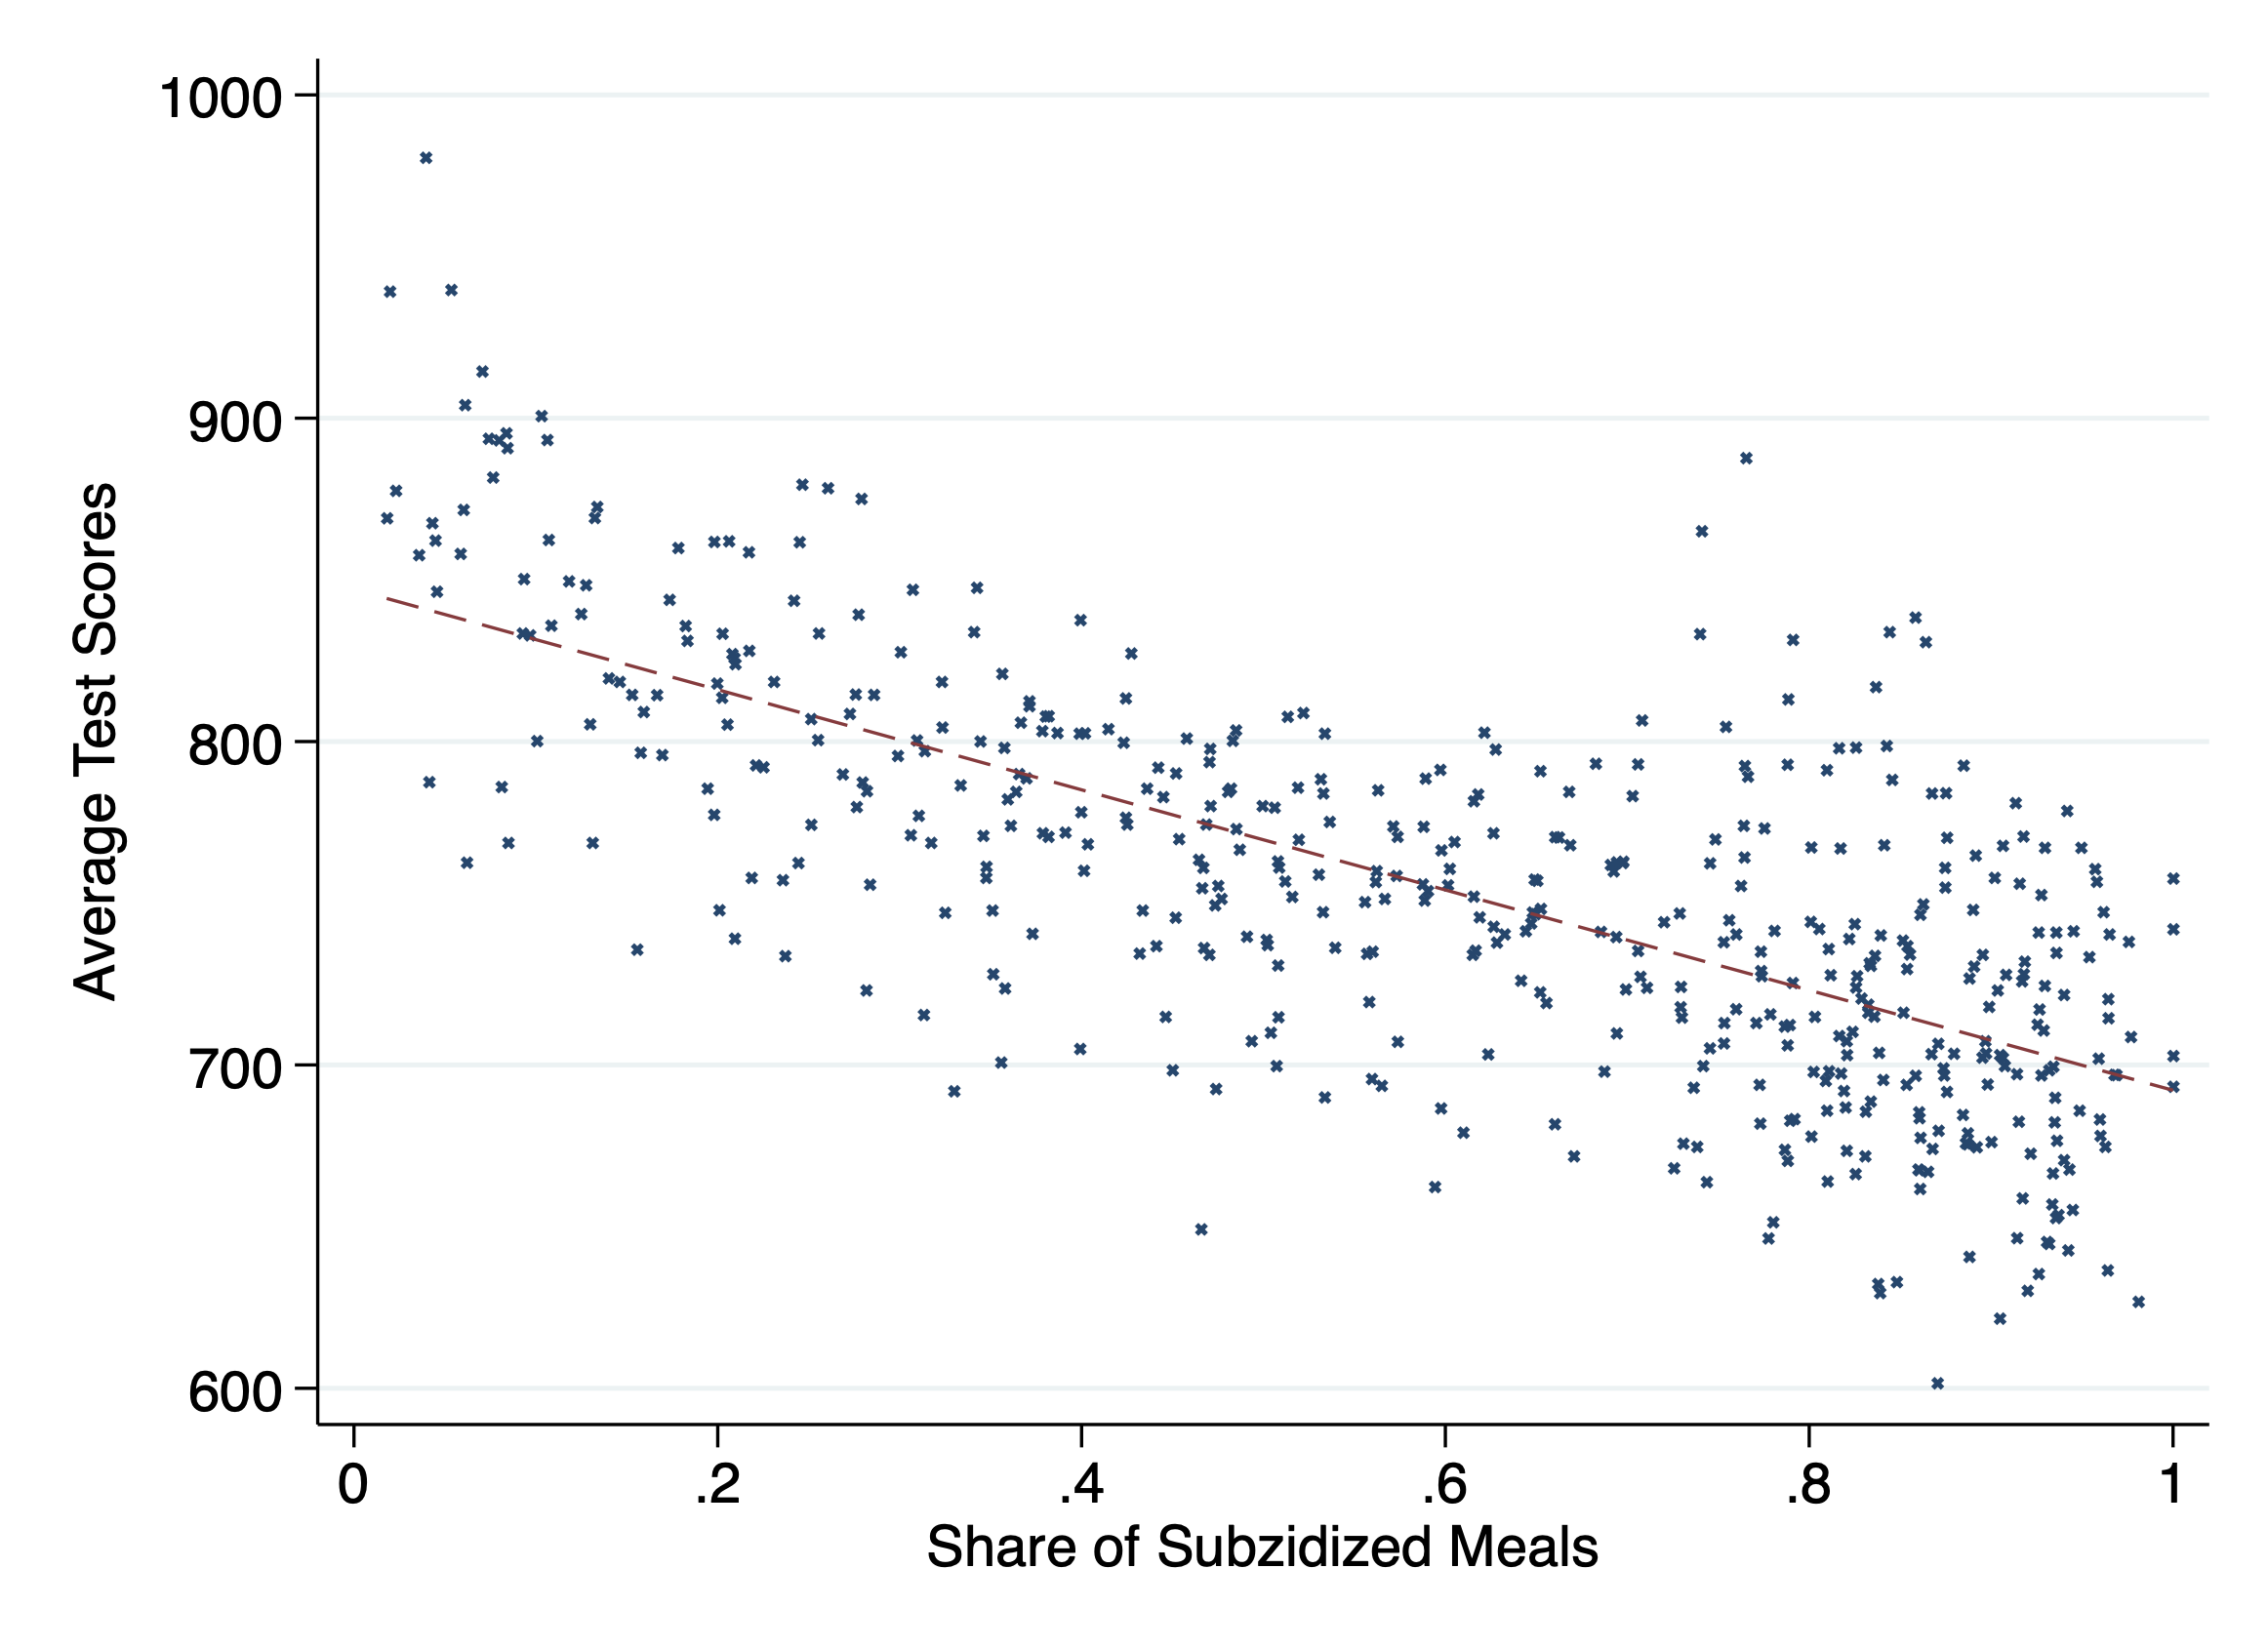
\includegraphics[scale=.25]{images/testscores_corr.png}
\end{figure}
\end{column}
\end{columns}
\end{frame}


\begin{frame}{The conditions for causality}
\begin{exampleblock}{The OLS Assumptions for Causal Inference}
Let
    \begin{equation*}
        Y_i  =  \beta_0 + \beta_1 X_i + u_i \text{~~;~~} i=1,...,n
    \end{equation*}
where $\beta_1$ is the causal effect of $X$ on $Y$. Then:
    \begin{enumerate}
        \item The error term $u_i$ has conditional mean $0$ given $X_i$: $\mathbb{E}(u_i\mid X_i)=0$;
        \item $(X_i, Y_i)$ $i=1,...,n$, are independent and identically distributed (i.i.d.) draws from their joint distribution; and
        \item Large outliers are unlikely: $X_i$ and $Y_i$ have nonzero finite fourth moments.
    \end{enumerate}
    
\end{exampleblock}
\end{frame}



\begin{frame}{The conditions for causality}
If these assumptions hold, then
\begin{enumerate}
    \item In large samples, the OLS estimators are consistent and have sampling distributions that are normal allowing for testing hypotheses and constructing confidence intervals
    \item They organize the circumstances that pose difficulties for OLS estimation of the causal effects
\begin{itemize}
    \item Assumption (1) ensures that $\hat{\beta}_1$ is an unbiased estimator of $\beta_1$
    \item Assumption (2) holds in cross-sectional contexts but is inappropriate for panel and time series data
    \item Assumption (3) reminds the importance of checking for large outliers
\end{itemize}
\end{enumerate}
\textit{Do you think these assumptions hold in our California Schools Experiment?}
\end{frame}



\begin{frame}{Assumption (1) : $\mathbb{E}(u_i\mid X_i)=0$}
 \begin{columns}
\begin{column}{0.35\textwidth}
\begin{itemize}
\item If \(E(u_i|X_i) \neq 0\), it implies that there is systematic variation in \(Y\) not explained by \(X\).
\item This unexplained variation can confound our causal interpretations, making it challenging to isolate the true causal effect of \(X\) on \(Y\).
\end{itemize}
\end{column}
\begin{column}{0.7\textwidth}
\begin{figure}
  \centering
         \vspace{-1mm}
        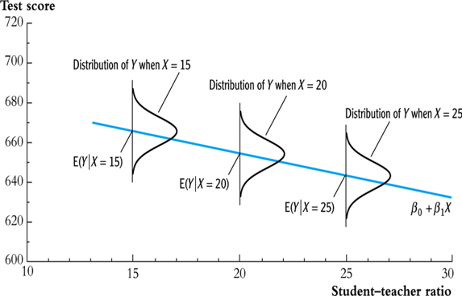
\includegraphics[scale=.75]{images/ols_assumption_1.png}
\end{figure}
\end{column}
\end{columns}
\end{frame}



\begin{frame}{Assumption (1) : $\mathbb{E}(u_i\mid X_i)=0$}
Remember that
\begin{equation*}
    \hat{\beta}_1= \frac{\frac{1}{n}\sum_{i=1}^n (Y_i-\overline{Y})(X_i - \overline{X})}{\frac{1}{n}\sum_{i=1}^n (X_i - \overline{X})^2} = \frac{s_{XY}}{s^2_x} = \frac{cov(X,Y)}{var(X)}
\end{equation*}

Then
\begin{eqnarray*}
    & \hat{\beta}_1 &= \frac{cov(X,[\beta_0 + \beta_1 X + u])}{var(X)}\\
    & &= \frac{cov(X,\beta_0)}{var(X)}+\frac{cov(X,\beta_1 X)}{var(X)}+\frac{cov(X,u)}{var(X)}\\
    & &= \beta_1+\frac{cov(X,u)}{var(X)}
\end{eqnarray*}
If $\mathbb{E}(u_i\mid X_i)\neq 0$, then $cov(X,u) \neq 0$... In the California Schools Experiment, schools subsidizing meals (vs. not) are likely to welcome students from poor (vs. rich) economic and social backgrounds -- biasing estimates downwards!
\end{frame}



\begin{frame}{Assumption (2): i.i.d. draws}
This arises automatically if the entity (individual, district) is sampled by simple random sampling:
\begin{itemize}
    \item The entities are selected from the same population, so $(X_i, Y_i)$  are identically distributed for all $i=1,...,n$.
    \item The entities are selected at random, so the values of $(X, Y)$ for different entities are independently distributed.
\end{itemize}
The main place we will encounter non-i.i.d. sampling is when data are recorded over time for the same entity (panel data and time series data) – we will deal with that complication when we cover panel data.
\end{frame}



\begin{frame}{Assumption (3): No large outliers}
 \begin{columns}
\begin{column}{0.35\textwidth}
\begin{itemize}
\item If $X$ and $Y$ are bounded, then they have finite fourth moments. (Standardized test scores automatically satisfy this; family income, etc. satisfy this too.)
\item The substance of this assumption is that a large outlier can strongly influence the results
\item Why is it an outlier? Is it a typo? In practice, outliers are often data glitches (coding or recording problems). If so, they really shouldn’t be in your data set!
\end{itemize}
\end{column}
\begin{column}{0.7\textwidth}
\begin{figure}
  \centering
         \vspace{-1mm}
        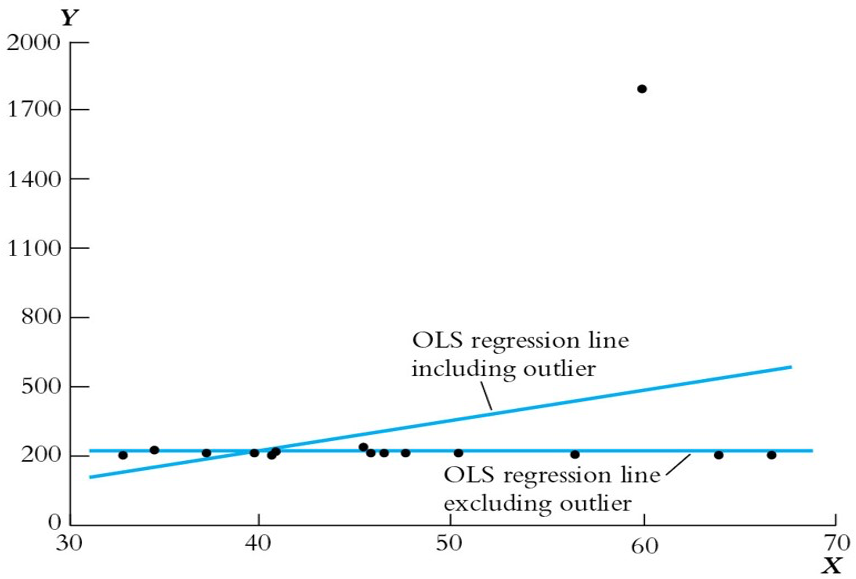
\includegraphics[scale=.6]{images/ols_assumption_2.png}
\end{figure}
\end{column}
\end{columns}
\end{frame}


\begin{frame}{OLS Sample Properties}
%Note that
\begin{eqnarray*}
&\hat{\beta}_1 &= \frac{\sum_{i=1}^n (X_i - \overline{X})(Y_i - \overline{Y}) }{\sum_{i=1}^n (X_i - \overline{X})^2}\\
& &= \frac{\sum_{i=1}^n (X_i - \overline{X})Y_i }{\sum_{i=1}^n (X_i - \overline{X})^2}\\
& &= \frac{\sum_{i=1}^n (X_i - \overline{X})(\beta_0 + \beta_1 X_i + u_i) }{\sum_{i=1}^n (X_i - \overline{X})^2}\\
& &= \frac{\beta_0\sum_{i=1}^n (X_i - \overline{X})+\beta_1 \sum_{i=1}^n (X_i - \overline{X}) X_i+\sum_{i=1}^n (X_i - \overline{X})u_i}{\sum_{i=1}^n (X_i - \overline{X})^2}\\
& &= \frac{\beta_1 \sum_{i=1}^n (X_i - \overline{X})(X_i - \overline{X})+\sum_{i=1}^n (X_i - \overline{X})u_i}{\sum_{i=1}^n (X_i - \overline{X})^2}\\
& &=\beta_1 +\frac{\sum_{i=1}^n (X_i - \overline{X})u_i}{\sum_{i=1}^n (X_i - \overline{X})^2}
\end{eqnarray*}

\end{frame}


\begin{frame}{OLS Sample Properties --- $\mathbb{E}[\hat{\beta}_1]$}
%Note that
\begin{eqnarray*}
&\mathbb{E}[\hat{\beta}_1] &=\mathbb{E}[\mathbb{E}[\hat{\beta}_1\mid X]] \\
& &=\beta_1  + \mathbb{E}\left[\mathbb{E}\left[\frac{\sum_{i=1}^n (X_i - \overline{X})u_i}{\sum_{i=1}^n (X_i - \overline{X})^2}\Big| X\right]\right] \\
& &=\beta_1  + \mathbb{E}\left[\frac{\mathbb{E}[\sum_{i=1}^n (X_i - \overline{X})u_i\mid X]}{\sum_{i=1}^n (X_i - \overline{X})^2}\right] \\
& &=\beta_1  + \mathbb{E}\left[\frac{\sum_{i=1}^n (X_i - \overline{X})\mathbb{E}[u_i\mid X]}{\sum_{i=1}^n (X_i - \overline{X})^2}\right] \\
& &=\beta_1  + \mathbb{E}\left[\frac{\sum_{i=1}^n (X_i - \overline{X})0}{\sum_{i=1}^n (X_i - \overline{X})^2}\right] \\
& &=\beta_1
\end{eqnarray*}
\end{frame}

\begin{frame}{OLS Finite Sample Properties --- $var[\hat{\beta}_1]$}
\begin{eqnarray*}
& var(\hat{\beta}_1 \mid X) =  var(\hat{\beta}_1 - \beta_1 \mid X) &= var\left[\frac{\sum_{i=1}^n (X_i - \overline{X})u_i}{\sum_{i=1}^n (X_i - \overline{X})^2}\Bigg|X\right]\\
& &= var\left[\frac{\sum_{i=1}^n (X_i - \overline{X})u_i}{TSS_X}\Bigg|X\right]\\
& &= \frac{1}{TSS_X^2}var\left[\sum_{i=1}^n (X_i - \overline{X})u_i\bigg|X\right]\\
& &= \frac{\sum_{i=1}^n (X_i - \overline{X})^2 var(u_i\mid X)}{TSS_X^2}\\
& &= \frac{\sigma^2_u}{TSS_X}\\
\end{eqnarray*}
By the law of total variance (i.e., variance decomposition formula)
\begin{eqnarray*}
     var(\hat{\beta}_1) = \mathbb{E}(var(\hat{\beta}_1 \mid X))+var(\mathbb{E}(\hat{\beta}_1 \mid X)) =  \mathbb{E}(var(\hat{\beta}_1 \mid X)) =   \frac{\sigma^2_u}{TSS_X}
\end{eqnarray*}
\end{frame}

% \begin{frame}{OLS Sample Properties --- $\mathbb{E}[\hat{\beta}_0]=\beta_0$}
% %Note that
% \begin{eqnarray*}
% &\mathbb{E}[\hat{\beta}_0] &=\mathbb{E}[\overline{Y}_i-\hat{\beta}_1\overline{X}] \\
% & &=\mathbb{E}[\beta_0 + \beta_1 \overline{X} + \frac{1}{n}\sum_{i=1}^n u_i -\hat{\beta}_1\overline{X}] \\
% & &=\beta_0 + \mathbb{E}(\beta_1 -\hat{\beta}_1) \overline{X} + \frac{1}{n}\sum_{i=1}^n \mathbb{E}(u_i)\\
% & &=\beta_0 + \frac{1}{n}\sum_{i=1}^n \mathbb{E}[\mathbb{E}(u_i\mid X)]\\
% & &=\beta_0 
% \end{eqnarray*}
% \end{frame}


\begin{frame}{OLS Finite Sample Properties --- $var[\hat{\beta}_1]$}
 \begin{columns}
\begin{column}{0.5\textwidth}
\begin{itemize}
    \item Here we made the assumption that $u$ is homoskedastic (i.e., it has the same variance given any value of the explanatory variable): $var(u_i\mid X)=\sigma^2_u~~\forall~~i$
    \item Note that a natural estimator of $var[\hat{\beta}_1]$, $\frac{\hat{\sigma}_u^2}{TSS_X}$ is $\frac{SSR}{(n-2) TSS_X}$.
    \item Larger error $u$ variance increases $Var(\hat{\beta}_1)$ since it makes it harder to estimate $\beta_1$ accurately.
\end{itemize}
\end{column}
\begin{column}{0.6\textwidth}
\begin{figure}
  \centering
         \vspace{-1mm}
        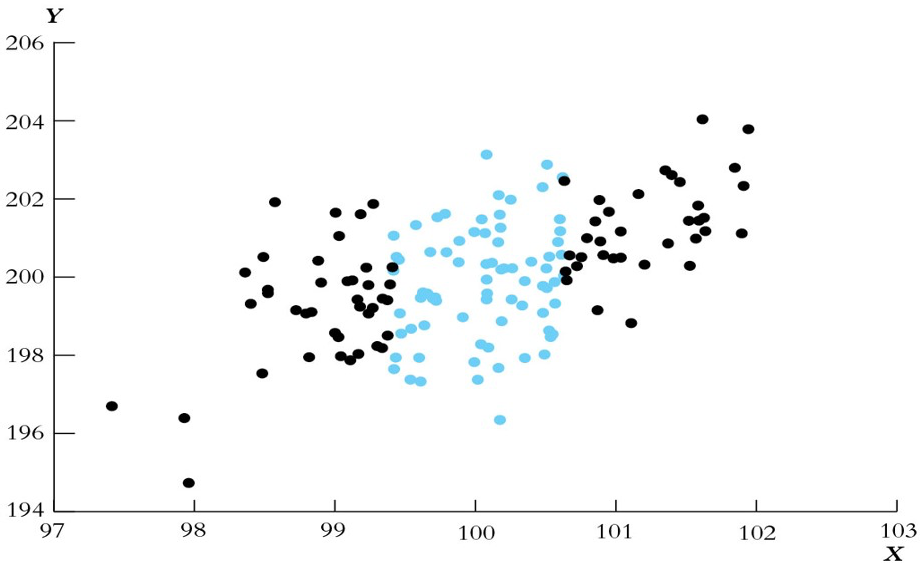
\includegraphics[scale=.4]{images/variance_x.png}
\end{figure}
\end{column}
\end{columns}
\begin{itemize}
    \item More variability in the independent variable ($X$) decreases the variance of $\hat{\beta}_1$ because it helps in estimating the relationship between $Y$ and $X$.
    \item  Increasing sample size reduces the variance of $\hat{\beta}_1$ as it captures more variation in $X$. 
    \item Ideally, we would choose $X$ to be as spread out as possible -- this is sometimes possible with experimental data, but in practice, we often work with random samples
\end{itemize}
\end{frame}



\begin{frame}{Large Sample Distribution of the OLS Estimator}
\begin{itemize}
    \item Other than its mean and variance, the exact distribution of $\hat{\beta}_1$ is complicated and depends on the distribution of $(X; u)$
    \item Because the $\mathbb{E}[\hat{\beta}_1] = \hat{\beta}_1$ and $var(\hat{\beta}_1)=0$ as $n\rightarrow \infty$, then, by the Law of Large Numbers, $\hat{\beta}_1 \xrightarrow[]{p} \beta_1$ (i.e., $\hat{\beta}_1$ is a consistent estimator of $\beta_1$)
    \item When $n$ is large, by the Central Limit Theorem, the sampling distribution of $\hat{\beta}_1$ is well approximated by a normal distribution $\mathcal{N}(\beta_1; \frac{\sigma^2_u}{TSS_X})$
    \item Said differently, $\frac{\hat{\beta}_1-\beta_1}{\sqrt{var(\hat{\beta}_1)}}\sim \mathcal{N}(0;1)$
    \item Note that this parallels the sampling distribution of $\overline{Y}!$
    \item We can use a similar reasoning with $\mathbb{E}[\hat{\beta}_0] = \hat{\beta}_0$ and that $var[\hat{\beta}_0] = \frac{\sigma^2_u \sum_{i=1}^n X_i}{n TSS_X}$
\end{itemize}\vspace{1cm}
$\Rightarrow$ We are now ready to tackle hypothesis testing with OLS!
\end{frame}



\begin{frame}[allowframebreaks]{Material}
\begin{itemize}
    \item[--] \textbf{Textbooks:}
    \begin{itemize}
        \item Introduction to Econometrics, 4th Edition, Global Edition, by Stock and Watson -- Chapter 4
    \end{itemize}
\end{itemize}
\end{frame}



\end{document}

